% -----------------------------------------------
% Vlastní text práce (kapitoly práce)
% -----------------------------------------------

% -----------------------------------------------
\chapter{Electronics for signal readout and analysis}
% -----------------------------------------------
The signals coming out of the detector need to be properly pre-amplified, amplified and shaped. This task requires special analogue circuits with a properly designed layout. 
The measurement chain for gamma spectroscopy is usually realised in the following order - gamma detector, preamplifier, amplifier, multichannel analyser (MCA), microprocessor/computer (figure \ref{chain}). When designing this spectrometric chain, we select components to achieve sufficient parameters for a particular application - in our case, energy resolution. For our spectrometric chain we chose instruments, modules and parts from two companies - ORTEC and CREMAT.
%The signals coming out of the detector have to be properly preamplified, amplified and shaped. This  task requires special analog circuits with properly designed layout. 
%The measurement chain for gamma spectroscopy is usually realized in following order - gamma detector, preamplifier, amplifier, multichannel analyser (MCA), microprocessor/computer (figure \ref{chain}). When designing this spectrometric chain, we select components in order to achieve sufficient parameters for certain application - in our case the energy resolution. For our spectrometric chain we chose instruments, modules and parts from two companies - ORTEC and CREMAT.

\begin{figure}[H]
 \centering
 \includegraphics[scale=0.35, angle = 0]{./pictures/chain.png}
 \caption{Spectrometric chain.}
 \label{chain}
 
\end{figure}


\par
The task of realising the spectrometric chain can be accomplished in two ways. The first and simpler way is to build it from stand-alone robust instruments and modules. The second way is to design a printed circuit board (PCB) with the required functionalities from electronic components. In this thesis we use both methods for the development. 
\par
Building the chain from stand-alone instruments can be a more practical approach for testing the detectors themselves, as we are not forced to solve problems arising from the design of the electronic circuit board. However, these modules are usually very expensive, the measurement setups build this way are unnecessarily large and have worse noise parameters than electronic circuits specially tailored for the given application.
\par
The PCB design requires a lot of electronic engineering skills and development time. The analog PCBs are very difficult to design. The advantages are that the final product can be very compact and cheap to manufacture.
%The task of realizing the spectrometric chain can be fulfilled in two ways. The first and more straightforward way is to build it from stand-alone robust instruments and modules. The second possibility is to design printed circuit board (PCB) with required functionalities from electronic components. In this thesis, we apply both methods for the development. 
%\par
%Building the chain from the stand-alone instruments can be more practical approach for testing of the detectors themselves since we are not forced to solve problems arising from the design of the board of the electronic circuit. However, these modules are usually very expensive, measurement setups build this way are unnecessarily large and have worse noise parameters than electronic circuits specially tailored for the given application.
%\par
%Designing the PCB requires many electronic engineering skills and time for development. The analog PCBs are very hard to design. The pros are that the final product can be very compact and cheap to manufacture.



\section{PIN detector connection and bias voltage}
\subsection{Voltage source}
The PN and PIN detectors require a voltage bias to reduce the capacitance.
These voltage sources don't need to be stiff as the current consumption of the detector is very low.
\par
Gas and scintillation detectors usually require high voltage sources (hundreds or thousands of volts). These high voltages are usually delivered by switching power supplies.
However, these supplies are usually very noisy, and since semiconductors can be operated at much lower voltages, they are not needed. The better alternative is to use charge pump built of capacitors and diodes, which require lower frequencies to operate.
%The PN and PIN detectors require voltage bias to reduce the capacitance.
%These voltage sources don't have to be stiff since the current consumption of the detector is very low.
%\par
%Gas and scintillation detectors usually require high voltage sources (hundreds or thousands of volts). These high voltages are usually delivered by switching power supplies.
%However, these supplies are usually very noisy and since the semiconductors can be operated at much lower voltages, there is no need for them. The better alternative is charge pump build of capacitors and diodes, which requires lower frequencies to operate.
\subsection{Shielding and grounding}
Electromagnetic shielding is a very important part of sensitive analog signal circuits. Sensitive circuits must be surrounded from all sides by a metallic material, which must also be correctly connected to GND (the principle of the Faraday cage), otherwise correct operation cannot be guaranteed. The electromagnetic disturbance usually induces currents in the shielding material, so special care must be taken to prevent these currents from flowing through the signal routes. The figure \ref{shielding} shows the difference between correct and incorrect shield connection.
%In case of sensitive analog signal circuits, the electromagnetic shielding is a very important part. Sensitive circuits have to be surrounded by a metallic material from all sides, which is also correctly connected to GND (principle of the Faraday cage), otherwise the proper functionality can not be guaranteed. The electromagnetic disturbance usually induces currents in the shielding material, and thus the special care has to be taken to prevent these currents from flowing through the signal routes. The figure \ref{shielding} shows the difference between correct and wrong connection of shielding.

\begin{figure}[H]
 \centering
 \includegraphics[scale=0.35, angle = 0]{./pictures/shielding.png}
 \caption{Schematic of incorrect and correct connection of shielding \cite{appCSPnote}.}
 \label{shielding}
 
\end{figure}



\subsection{Cooling}
To reduce thermal noise and achieve better SNR, it is necessary to cool the detector. Cooling can be achieved in a number of ways. In most setups, a Peltier cooler can provide the appropriate solution. These Peltier setups are the easiest to implement, but their cooling efficiency is highly dependent on the ability to sink the heat from the hot side.
%To reduce thermal noise and achieve better SNR it is necessary to cool the detector. The cooling can be achieved by various ways. In most setups, the appropriate solution can be provided by a Peltier cooler. These setups with Peltier are the easy to implement, however, their cooling efficiency is highly dependent on the ability to sink the heat from the hot side.

\section{Spectrometric chain components}
\subsection{Pre-amplification}
The signal coming from the PIN detector is a charge (current pulse), so it is necessary to convert it into a voltage pulse. To perform the charge-voltage conversion, there is a circuit called a charge amplifier (also called a preamplifier). The main functional scheme is described by an opamp with a capacitor in feedback (see figure \ref{trans}). The functionality is similar to an $I/U$ transimpedance amplifier, but the charge amplifier works mainly as an integrator. In the ideal case (opamp gain $A >> 0$) the measured voltage per unit charge is approximately equal to:
%The signal coming out of the PIN detector is a charge (current pulse), so it is necessary to convert it into voltage pulse. For performing the charge-voltage conversion, there is circuit called charge amplifier (also referred as a preamplifier). The principal functional scheme is described by one opamp with a capacitor in feedback (see figure \ref{trans}). The functionality is similar to $I/U$ transimpedance amplifier, but the charge amplifier works mainly as an integrator. In ideal case (opamp amplification $A >> 0$), the measured voltage per unit charge is approximately equal to:

\begin{equation}
\frac{dU}{dQ} = \frac{1}{C_{f}}.
\end{equation}
\par
In a real circuit there is also a resistor in parallel with the feedback capacitor. The feedback resistor slowly discharges the capacitor after an accumulation of charge, making the transimpedance amplifier ready to capture another pulse. The output voltage has an exponential decay shape with amplitude defined by the energy deposited in the detector, a short rise time (in the order of nanoseconds) and a longer decay constant (microseconds). Since the output of the preamplifier is in the order of millivolts, it must be highly amplified. A very fast and low-noise amplifier consisting of several opamps is a suitable solution to this problem. Charge preamplifiers are also very sensitive devices and can be easily damaged by electrostatic charges. 
%\par
%In real circuit there is also a resistor parallel to the feedback capacitor. The feedback resistor slowly discharges the capacitor after a accumulation of charge, restoring the transimpedance amplifier to be ready to capture another pulse. The output voltage has the shape of exponential decay with amplitude defined by energy deposited into detector, short rise time (in orders of nanoseconds) and a longer decay constant (microseconds). Since the output of preamplifier is in order of millivolts, it has to be strongly amplified. Very fast and low noise amplifier consisting of multiple opamps is an appropriate solution of this problem. Charge preamplifiers are also very sensitive devices and can be very easily damaged by electrostatics. 

\begin{figure}[H]
 \centering
 \includegraphics[scale=0.4, angle = 0]{./pictures/champlifier.png}
 \caption{Charge ampifier. $Qs$ is total charge of pulse and $to$ is the interval of charge generation inside the detector. Taken from \cite{charge}.}
 \label{trans} 
\end{figure}
\begin{figure}[H]
 \centering
 \includegraphics[scale=0.4, angle = 0]{./pictures/NoiseEquiv.png}
 \caption{Noise equivalent circuit for charge amplifier. Taken from \cite{charge}.}
 \label{transNoise} 
\end{figure}
The functionality of the charge amplifier is also negatively affected by electronic noise, which depends on the values of the feedback resistance and capacitance, as well as on the internal parameters of the connected semiconductor detector and the field effect transistor (FET) inside the amplifier. The noise model of the preamplifier circuit is shown in the figure \ref{transNoise}. This electronic noise can be divided into three contributions, each described by equations for noise voltages and currents \cite{charge}:
%The functionality of charge amplifier is also negatively affected by an electronic noise, which depends on the values of the feedback resistance and capacitance and also on the internal parameters of the connected semiconductor detector and field-effect transistor (FET) inside the amplifier. The noise model of the preamplifier circuit can be seen in the figure \ref{transNoise}. This electronic noise can be divided into three contributions, each described by euqations for noise voltages and currents \cite{charge}:

% on including the detector's capacitance $C_{\textrm{det}}$. Thermal noise dependency on $C_{\textrm{det}}$ of the first-stage FET transistor can be approximated by equation \cite{charge}:
\begin{itemize}
\item Thermal noise of the first stage FET:
\begin{equation}
en_1 = \sqrt{\frac{8}{3}\frac{kT}{g_{\textrm{m}}}},
\end{equation}
where $k$ is the Boltzmann constant, $T$ is the absolute temperature and $g_{\textrm{m}}$ is the transconductance of the FET.
\item Shot noise caused by FET gate current and detector dark current:
\begin{equation}
in = \sqrt{2e(I_{\textrm{G}} + I_{\textrm{D}})},
\end{equation}
where $e$ is the elementary charge, $I_{\textrm{G}}$ is the gate leakage current of the first stage FET and $I_{\textrm{D}}$ is the dark current of the detector.
\item Thermal noise caused by feedback resistance: 
\begin{equation}
en_2 = \sqrt{4KTR_{\textrm{f}}},
\end{equation}
where $R_{\textrm{f}}$ is the feedback resistance.
\end{itemize}
The square of total noise $ent^2(j \omega)$ is given by equation:
\begin{equation}
\begin{aligned}
ent^2(j \omega) = en_1^2 \cdot (1+\frac{C_{\textrm{in}}}{C_{\textrm{f}}})^2 + \{in^2 + (\frac{en_2}{R_{\textrm{f}}})^2 \}\frac{1}{(j \omega C_{\textrm{f}})^2},
\end{aligned}
\label{finalNoise}
\end{equation}
where $C_{\textrm{f}}$ is the feedback capacitance, $C_{\textrm{in}}$ is the resulting capacitance at the amplifier input (there - parallel combination of the detector capacitance $C_{\textrm{j}}$ and the amplifier input capacitance $C_{\textrm{s}}$), $\omega$ is the angular frequency and $j$ is the complex unit.
\par
The first term in the equation \ref{finalNoise} depends on the ratio between the input capacitance $C_{\textrm{in}}$ and the feedback capacitance $C_{\textrm{f}}$, so the feedback capacitance of the preamplifier must be optimised to reduce the electronic noise.
\par
For the PCB design we used a CR-110-R2 charge amplifier from Cremat Inc. This preamplifier also contains the second stage - the common voltage amplifier.
CR-110-R2 offers the conversion gain $G = 1.4$ V/pC, decay constant $\tau = 140$ $\mu$s CR-110-R2) and noise (FWHM) in silicon equal to 1.7 keV \cite{cr110}. It can be easily calculated that for a 14.4 keV photon, the output pulse has an amplitude equal to $U_{A} = 0.8928$ mV. Note that the noise introduced by the preamplifier is much larger than the intrinsic Fano noise (FWHM = 185.4 eV).  Its internal scheme can be seen in the figure \ref{internal}.   
%\par
%The first term in equation \ref{finalNoise} depends on the ration between the input capacitance $C_{\textrm{in}}$ and the feedback capacitance $C_{\textrm{f}}$ and thus the preamplifier's feedback capacitance has to be optimized in order to reduce the electronic noise.
%\par
%In case of PCB design we used CR-110-R2 charge amplifier made by Cremat Inc. This preamplifier also contains the second stage - common voltage amplifier.
%CR-110-R2 offers the conversion gain $G = 1.4$ V/pC, decay constant $\tau = 140$ $\mu$s CR-110-R2) and noise (FWHM) in silicon equal to 1.7 keV \cite{cr110}. It can be easily calculated, that for 14.4 keV photon, the output pulse has amplitude equal to $U_{A} = 0.8928$ mV. Note that the noise caused by the preamplifier is much larger than the intrinsic fano noise (FWHM = 185.4 eV).  Its internal scheme can be seen in the figure \ref{internal}.

\begin{figure}[H]
 \centering
 \includegraphics[scale=0.35, angle = 0]{./pictures/CRpreamp.png}
 \caption{Internal scheme of CR-110-R2 charge sensitive preamplifier \cite{cr110}.}
 \label{internal}
 
\end{figure}
\par
The modular version suitable for our application is the ORTEC 142A charge preamplifier with $G = 1.016$ V/pC, $\tau = 500$ $\mu$s and noise in silicon equal to 1.6 keV \cite{ORTECpreamp}.

\subsection{Shaping}
To perform accurate energy discrimination, the pulse shape must be changed from an exponential decay shape by a shaping circuit. Shaping results in filtering the frequency band (reducing noise) and also shortens the long decay times of the original exponential shapes. The shorter duration of the pulses prevents the negative effect of one pulse being superimposed on another one (pile-up effect).

\par
The Gaussian shape satisfies the optimum parameters of SNR and duration \cite{Shapflify}. This type of shaping is usually achieved by several integration stages. The Cremat module CR-200-1us-R2.1 offers Gaussian shaping with a shaping time of 1 $\mu$s \cite{cr200}. Its simplified internal schematic is shown in the figure \ref{internal2}.  
%To perform the accurate energy discrimination, the pulse shape has to be altered from exponential decay shape by a shaping circuit. The shaping results into filtering the frequency band (reducing the noise) and also into shortening the long decay times of original exponential shapes. The shorter duration of pulses prevents the negative effect in which is one pulse superimposed onto another one (pile-up effect).
%
%\par
%The Gaussian shape meets the optimum parameters of SNR and duration \cite{Shapflify}. This type of shaping is usually achieved by several integration stages. The Cremat module CR-200-1us-R2.1 offers gaussian shaping with shaping time 1 $\mu$s \cite{cr200}. Its simplified internal schematic can be seen on fig.\ref{internal2}. 


\begin{figure}[H]
 \centering
 \includegraphics[scale=0.35, angle = 0]{./pictures/CRshaper.png}
 \caption{Internal scheme of CR-200 Gaussian shaping amplifier \cite{cr200}.}
 \label{internal2}
 
\end{figure}
The shapers are usually very sensitive to the shape of the input pulse. They expect a step-like input pulse. The deviation from the expected shape can result in an undefined shape at the output of the shaper.
%The shapers are usually very sensitive to the shape of the input pulse. They expect step-like input pulse. The deviation from the expected shape may result into undefined shape on output of the shaper.

\subsection{Multichannel analysis (MCA)}
To obtain full energy spectrum information, it is necessary to measure and digitise the pulse height of the incoming pulses to perform energy discrimination and increment the corresponding channels. The multichannel analyser (MCA) can be used for this purpose. The EASY-MCA-2K from ORTEC \cite{MCAOrtec}, which we are using in the experiments, is capable of processing Gaussian shaped pulses with shaping times from 0.25 $\mu$s to 30 $\mu$s and amplitudes from 0 to +10 V.
%To obtain the full energy spectra information, it is necessary to measure and digitize pulse height of incoming pulses to perform energy discrimination and increment the corresponding channels. The multichannel analyser (MCA) can be employed for these purposes. The EASY-MCA-2K from ORTEC \cite{MCAOrtec}, which we use in experiments, is capable of processing Gaussian shaped pulses with shaping times from 0.25 $\mu$s to 30 $\mu$s and amplitudes ranging from 0 to +10 V.



% %%%%%%%%%%%%%%%%%%%%%%%% End of file %%%%%%%%%%%%%%%%%%%%%%%%